%%%%%%%%%%%%%%%%%%%%%%% file template.tex %%%%%%%%%%%%%%%%%%%%%%%%%
%
% This is a general template file for the LaTeX package SVJour3
% for Springer journals.          Springer Heidelberg 2010/09/16
%
% Copy it to a new file with a new name and use it as the basis
% for your article. Delete % signs as needed.
%
% This template includes a few options for different layouts and
% content for various journals. Please consult a previous issue of
% your journal as needed.
%
%%%%%%%%%%%%%%%%%%%%%%%%%%%%%%%%%%%%%%%%%%%%%%%%%%%%%%%%%%%%%%%%%%%
%
% First comes an example EPS file -- just ignore it and
% proceed on the \documentclass line
% your LaTeX will extract the file if required
\begin{filecontents*}{example.eps}
%!PS-Adobe-3.0 EPSF-3.0
%%BoundingBox: 19 19 221 221
%%CreationDate: Mon Sep 29 1997
%%Creator: programmed by hand (JK)
%%EndComments
gsave
newpath
  20 20 moveto
  20 220 lineto
  220 220 lineto
  220 20 lineto
closepath
2 setlinewidth
gsave
  .4 setgray fill
grestore
stroke
grestore
\end{filecontents*}
%
\RequirePackage{fix-cm}
%
%\documentclass{svjour3}                     % onecolumn (standard format)
%\documentclass[smallcondensed]{svjour3}     % onecolumn (ditto)
\documentclass[smallextended]{svjour3}       % onecolumn (second format)
%\documentclass[twocolumn]{svjour3}          % twocolumn
%
\smartqed  % flush right qed marks, e.g. at end of proof
%
\usepackage{graphicx}
%
% \usepackage{mathptmx}      % use Times fonts if available on your TeX system
%
% insert here the call for the packages your document requires
%\usepackage{latexsym}
% etc.
%
% please place your own definitions here and don't use \def but
% \newcommand{}{}
%
% Insert the name of "your journal" with
% \journalname{myjournal}
%
\begin{document}

\title{Blind prediction of cyclohexane-water distribution coefficients from the SAMPL5 challenge}
\thanks{NSF, green planet (their NSF), anything else?}

\subtitle{I don't think we need a subtitle...}

%\titlerunning{Short form of title}        % if too long for running head

\author{Caitlin C Bannan         \and
        Kalistyn H Burley \and
        David L Mobley
}

%\authorrunning{Short form of author list} % if too long for running head

\institute{C. C. Bannan, K. H. Burley, and D. L. Mobley \at University of California, Irvine \\
              Tel.: +123-45-678910\\
              Fax: +123-45-678910\\
              \email{dmobley@mobleylab.org}           %  \\
%             \emph{Present address:} of F. Author  %  if needed
}

\date{Received: date / Accepted: date}
% The correct dates will be entered by the editor


\maketitle

\begin{abstract}
% Add an abstract
% Add to keywords
\keywords{distribution coefficient \and blind challenge \and free energy } 
% \PACS{PACS code1 \and PACS code2 \and more}
% \subclass{MSC code1 \and MSC code2 \and more}
\end{abstract}

% For now what I have done is filled in headings and a sentence to describe each paragraph in each section. It looks like with JCAMD we can use any section headings we like so I've tried to stick with the titles as statements concept. 


\section{Introduction}
\label{intro}
SAMPL is a blind challenge, has included solvation free energy in the past

What is a distribution coefficient? Relate to free energy, distiguish from logP

% I'm looking to see if there are blind challenges that have used logP or logD 
More detail about why logD

Possibly brief statement about samples set, site Bas' experimental paper. We provide a detailed look at our submissions to the SAMPL5 challenge and an analysis of submitted results


\section{Challenge Logistics}
\label{logistics}
Timeline and how many total participants - assigned 2 digit i.d, option to be anonomous, worshop

Number of molecules, organized into batches with sizes (submit 0, 0-1, or 0-2), what was provided to participants

Reporting logD in cyclohexane/water (where water is aq. buffer), explain two different uncertainties

We did not have access to experimental results and participated Blind in the challenge, possibly comment on distribution of work (i.e. KHB doing calculations and CCB doing analysis)

% the next three sections, I thought of as "methods" but I'm titling them with more detail
\section{Error metrics and ...}
\label{analysis}
Error metrics considered, bootstrapping to estimate uncertainty

QQ plots and what 'error slope' is

% number of tautomers? checkmol molecules? Kendall W? 

\section{Submissions from the Mobley Group}
\label{methods:1}
\paragraph{partition coefficient from solvation free energies}
Submission 39 done by KHB blind, following protocol established in the group to calculate logP % Cite Caitlin's paper? 
Probably one more paragraph detailing those methods, GAFF AM1-BCC, GROMACS, etc.

As a part of this study, we also wanted to varify that a change in box size does not affect the calculated solvation free energy with solvents of a low dielectric constant, such as cyclohexane. 
Previously, the Mobley group showed that there was no significant change in calculated hydration free energies for small polar compounds in 2 to 9 nm water boxes.  

\paragraph{Null Hypothesis}
% I need to find a good citation, but I remember talking in Pharm 272 about how a "good" predictive method should do better than any null hypothesis. 

good predictive method should be better than a "null" hypothesis. All molecules equally distribute between cyc and water so logD = 0.0

\paragraph{...} % Something like empirical prediction or fast regression method... 
All common partition coefficient predictors are for octanol/water, what if you just assumed that was logDcyc or that you could correct that with a simple bias correction?

\subsection{Consideration of tautomers after SAMPL}
\label{methods:post}
corrections based on pKa

corrections based on tautomer enumeration

\section{Results and Discussion}
\label{results:1}
To compare each prediction set to experiment compare plots, QQ, error metric calculated for each prediction set

To visualize how prediction sets compared to each other, explain histograms

Some submissions did not include batch 1 or 2, how many of each and approximately where they were on the histograms...

Error Slope, only one group (2 submissions) did a good job with this % cite Andrew Paluch's paper if he is writing one

% Kendall W if we decide to include it

\subsection{Prediction sets that performed most strongly}
\label{results:2}
We want to consider how close to experiment RMSE/AUE and how well correlated with experiment tau/R

16 did best across both metric, COSMO-RS, brief statement about procedure

14 and 36 also did very well, making "top 10" by at least 3 of those 4 metrics, 14 is one of Frank Pickard's and 36 is Chris Fennell

but really null did best across the board so we have a lot of work to do... best RMSE over 2.0 log units and average around 3.5

\subsection{Compounds that were difficult to accurately predict}
\label{results:3}
Full error analysis repeated for individual molecules, there aren't very many "simple" molecules, almost all have hetro atoms and rotatable bonds...

~5-10 worst, I'm looking into if there are # of tuatomer or functional group similarities...

~5-10 best, still looking for trends, we know 083, 074. 015 also did poorly. 

% possibly a paragraph about MW, # of rotatable bonds, or # of tautomers (no tautomer trend yet...)

\subsection{Classes of methods...}
\label{results:4}
Broad range of methods, split into classes: MD all atom, MD hybrid, quantum?, Anything similar to COSMO? % I'm still reading and trying to understand methods
Pie chart by number maybe?

Clear trends on which are doing well? 

\subsection{Mobley group prediction results}
\label{results:5}
How did logP do, not bad in general, include our plots

Slight bias for cyclohexane over water, probably because tautomer enumeration will increase concentrations in water?

pKa corrections
tautomer corrections

Biases, and major shifts for some compounds - tautomers in cyclohexane not being accounted for

\subsection{Reanalysis of difficult tautomers} % I don't like difficult here
\label{results:6}
It was clear from epik and discussions with other SAMPL5 participants (cite Klamt?)  that 050 and 083 had dominant tautomers other than provided SMILE

We reran these tautomers to calculate solvation free energies, used state penalty %results in a table probably (or maybe a figure like the one I made for erythromycin in the logP paper)

Generally hard to tell if its tautomer enumeration that isn't good or the solvation free energies

\section{Conclustion}
\label{conclusions}

Overall, range of methods and performance

Compare to dGhydration in past SAMPL challenges? using average errors, possibly what methods/FF are top ranked?

Tautomer and/or pKa predictions are going to be an important part of improving these

We, as a communitte, need to improve error estimation, both how we do and how we evaluate it...

logP/logD seem to be good options for future blind challenges

\begin{acknowledgements} % this is just a list so we don't forget anyone
John Chodera and Bas MSKCC
Andreas Klamt
Chris Fennell
Samuel Genheden
D3R team
people who set up the automated submission system %they are gods in my opion =]


\end{acknowledgements}

\subsection{Available in supporting info} % This is a list for myself, it will all be zipped or provided with a link to to somewhere on the web
things provided to participants
all scripts used for error analysis
all participant files? Can we include the anonomous one? 
triple check no names/e-mails/institutions/etc in the final submitted data
all plots not in the paper
all input/output files for schrodinger calculations
all input files and results files for 'logP' calculations, tautomer redos, box size simulations (PME too?) 
example MDP and run scripts
 


% BibTeX users please use one of
%\bibliographystyle{spbasic}      % basic style, author-year citations
%\bibliographystyle{spmpsci}      % mathematics and physical sciences
%\bibliographystyle{spphys}       % APS-like style for physics
%\bibliography{}   % name your BibTeX data base

%\subsection{Subsection title}
%\label{sec:2}
% Examples from the JCAMD template 
% Text with citations \cite{RefB} and \cite{RefJ}.
% (see Sect.~\ref{sec:1}).
% \paragraph{Paragraph headings} Use paragraph headings as needed.

% For one-column wide figures use
%\begin{figure}
% Use the relevant command to insert your figure file.
% For example, with the graphicx package use
%  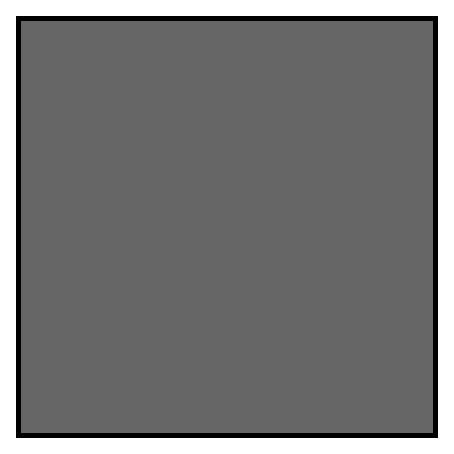
\includegraphics{example.eps}
% figure caption is below the figure
%\caption{Please write your figure caption here}
%\label{fig:1}       % Give a unique label
%\end{figure}
%
% For two-column wide figures use
%\begin{figure*}
% Use the relevant command to insert your figure file.
% For example, with the graphicx package use
%  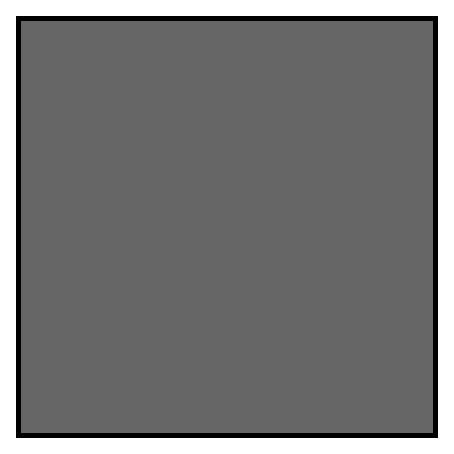
\includegraphics[width=0.75\textwidth]{example.eps}
% figure caption is below the figure
%\caption{Please write your figure caption here}
%\label{fig:2}       % Give a unique label
%\end{figure*}
%
% For tables use
%\begin{table}
% table caption is above the table
%\caption{Please write your table caption here}
%\label{tab:1}       % Give a unique label
% For LaTeX tables use
%\begin{tabular}{lll}
%\hline\noalign{\smallskip}
%first & second & third  \\
%\noalign{\smallskip}\hline\noalign{\smallskip}
%number & number & number \\
%number & number & number \\
%\noalign{\smallskip}\hline
%\end{tabular}
%\end{table}


\end{document}

